\documentclass[12pt, a4paper]{report}

\usepackage[utf8]{inputenc}
\usepackage{geometry}
 \geometry{
 a4paper,
 total={170mm,257mm},
 left=20mm,
 top=20mm,
}

\usepackage{titlesec}
\titleformat
{\chapter}
[display]{\bfseries\Large\itshape}
{Capitolo Nr.\thechapter}
{0.5ex}
{
    \rule{\textwidth}{1pt}
    \vspace{1ex}
	\centering
}
[\vspace{-0.5ex}\rule{\textwidth}{0.3pt}]

\usepackage{titling}
\newcommand{\subtitle}[1]{%
  \posttitle{%
    \par\end{center}
    \begin{center}\large#1\end{center}
    \vskip0.5em}%
}

\renewcommand{\contentsname}{Indice}

\usepackage{amsthm} % Fornisce il comando \newtheorem
\usepackage{thmtools} % fornisce il comando \declaretheorem
\usepackage{amsmath}
\usepackage{amsfonts}
\usepackage{amssymb}
\usepackage{enumitem} % Permette di usare la numerazione romana nelle liste
\usepackage{latexsym}
\usepackage{mathtools}
\usepackage{dsfont}
\usepackage{tikz}

\theoremstyle{definition}
\newtheorem{definition}{Definizione}[section]
\newtheorem{theorem}{Teorema}[section]
\newtheorem{corollary}{Corollario}[theorem]
\newtheorem{lemma}{Lemma}[theorem]
\newtheorem{observation}{Oss}[section]
\declaretheorem[name=Dim, qed=$\blacksquare$, numbered=no]{demonstration}
\newtheorem*{proposition}{Prop}
\newtheorem*{property}{Proprietà}
\newtheorem*{note}{NB}

\newcommand{\Mod}[1]{\ (\mathrm{mod}\ #1)}
\newcommand{\inv}{(\mathbb{Z}/n\mathbb{Z})^*}

\title{Svolgimento esame di Fondamenti matematici per l'informatica}
\author{Leonardo De Faveri}
\date{23 giugno 2021}

\begin{document}
\maketitle
\paragraph{Esercizio 1)}
Si dimostri per induzione che, per ogni intero $n\geq2$, vale:
\[\sum_{k=2}^n\frac{k-1}{2^k}=1-\frac{n+1}{2^n}\]
\subparagraph{Soluzione:}
Procedo per induzione su $n\geq2$.
\begin{itemize}
    \item $n=2$ (\emph{Base dell'induzione}): dimostro che vale $\sum_{k=2}^2
    \frac{k-1}{2^k}=1-\frac{2+1}{2^2}$
    \setlength\arraycolsep{30pt}
    \[\begin{array}{cc}
        \bullet\sum_{k=2}^2\frac{k-1}{2^k}=\frac{2-1}{2^2}=\frac{1}{4}
        &\bullet 1-\frac{2+1}{2^2}=1-\frac{3}{4}=\frac{1}{4}
    \end{array}\]
    La base dell'induzione è verificata.
    \item $n\geq2\Rightarrow n+1$ (\emph{Passo induttivo}): ipotizzo che
    l'uguaglianza sia vera per un qualche $n\geq2$, cioè che valga:
    \[\sum_{k=2}^n\frac{k-1}{2^k}=1-\frac{n+1}{2^n}\text{ per qualche }n\geq2\
    (\text{Ip. Ind.})\]
    Dimostro che la stessa uguaglianza vale anche per $n+1$, ovvero dimostro che
    vale anche:
    \[\sum_{k=2}^{n+1}\frac{k-1}{2^k}=1-\frac{(n+1)+1}{2^{n+1}}\]
    Vale:
    \[\sum_{k=2}^{n+1}\frac{k-1}{2^k}=1-\frac{(n+1)+1}{2^{n+1}}\Leftrightarrow
    \frac{(n+1)-1}{2^{n+1}}+\sum_{k=2}^n\frac{k-1}{2^k}=1-\frac{n+2}{2^{n+1}}\]
    \[\Leftrightarrow\sum_{k=2}^n\frac{k-1}{2^k}=1-\frac{n+2}{2^{n+1}}-\frac{n}
    {2^{n+1}}\xLeftrightarrow{\text{Ip. Ind.}}1-\frac{n+1}{2^n}=1-\frac{2n+2}{2^{n+1}}\]
    \[\Leftrightarrow\frac{n+1}{2^n}=\frac{2(n+1)}{2^n\cdot2}\Leftrightarrow
    \frac{n+1}{2^n}=\frac{n+1}{2^n}\Leftrightarrow0=0\]
    L'identità $0=0$ è vera, quindi il passo induttivo risulta verificato, dunque
    per il teorema d'induzione, l'uguaglianza
    \[\sum_{k=2}^n\frac{k-1}{2^k}=1-\frac{n+1}{2^n}\]
    è vera per ogni intero $n\geq2$.
\end{itemize}

\newpage
\paragraph{Esercizio 2)}
Si determinino tutte le soluzioni del seguente sistema di congruenze:
\[\begin{cases}
    x\equiv45\Mod{77}\\
    x\equiv59\Mod{140}
\end{cases}\]
Si dimostri inoltre che non esiste alcuna soluzione positiva del suddetto sistema
che abbia una cifra pari al posto delle decine.
\subparagraph{Soluzione:}
Sia $S$ l'insieme delle soluzioni.
\begin{enumerate}[label={\arabic*$^o$}]
    \item Passo) \emph{Compatibilità}\\
    Grazie al Teorema cinese del resto so che il sistema di congruenze in questione
    è compatibile se e solo se $(140,77)|59-45$.\\
    Calcolo $(140,77)$:
    \[\begin{array}[t]{c|c}
        140 & 2\\
        70 & 2\\
        35 & 2\\
        7 & 7\\
        1
    \end{array}
    \begin{array}[t]{c|c}
        77 & 7\\
        11 & 11\\
        1
    \end{array}\]
    Poiché $140=2^2\cdot5\cdot7$ e $77=7\cdot11$, $(140,70)=7$. Dato che $59-45=
    14=2\cdot7$, $(140,70)=7|14=59-45$. Quindi, per il Teorema cinese del resto,
    il sistema è compatibile, ovvero $S\neq\emptyset$.\\
    Inoltre vale:
    \[59-45=14=2\cdot7=2\cdot(140,77)\]
    cioè
    \begin{equation}\label{eq:1}
        59-45=2\cdot(140,77)
    \end{equation}
    \item Passo) \emph{Calcolo di una soluzione}\\
    Applico l'algoritmo di Euclide con sostituzione a ritroso a $140$ e $77$:
    \[\begin{array}{rcl|rcl}
        140 &= &1\cdot77+63 & 63 &= &140-1\cdot77\\
        77 &= &1\cdot63+14 & 14 &= &77-1\cdot63\\
        63 &= &4\cdot14+7 & 7 &= &63-4\cdot14\begin{array}[t]{rcl}
            &= &63-4\cdot(77-1\cdot63)\\
            &= &5\cdot63-4\cdot77\\
            &= &5\cdot(140-1\cdot77)-4\cdot77\\
            &= &5\cdot140-9\cdot77
        \end{array}\\
        14 &= &2\cdot7+0
    \end{array}\]
    Ovvero vale:
    \begin{equation}\label{eq:2}
        7=5\cdot140+(-9)\cdot77\Leftrightarrow(140,77)=5\cdot140+(-9)\cdot77
    \end{equation}
    Grazie a (\ref{eq:1}) e (\ref{eq:2}) vale:
    \[59-45\overset{(\ref{eq:1})}{=}2\cdot(140,77)\overset{(\ref{eq:2})}{=}2\cdot
    (5\cdot140+(-9)\cdot77)=10.\cdot140+(-18)\cdot77\]
    ovvero
    \begin{equation}\label{eq:3}
        59-45=10\cdot140+(-18)\cdot77
    \end{equation}
    Da (\ref{eq:3}) deriva che
    \[\begin{array}{rcl}
        59-10\cdot140 &= &45-18\cdot77\\
        -1341 &= &-1341
    \end{array}\]
    Di conseguenza $c\coloneqq-1341$ è una soluzione del sistema.
    \item Passo) \emph{Calcolo di $S$}\\
    Grazie al Teorema cinese del resto so che l'insieme delle soluzioni $S$ è:
    \[S=[c]_{[140,77]}=[-1341]_{[140,77]}\subset\mathbb{Z}\]
    Calcolo $[140,77]$:
    \[[140,77]=\frac{140\cdot77}{(140,77)}=\frac{140\cdot77}{7}=140\cdot11=1540\]
    Dunque:
    \[S=[-1341]_{1540}=[-1341+1\cdot1540]_{1540}=[199]_{1540}\subset\mathbb{Z}\]
\end{enumerate}
\subparagraph{Seconda domanda:}
poiché le soluzioni del sistema sono tutti e soli i valori contenuti in:
\[S=\{199+k\cdot1540\ |\ k\in\mathbb{Z}\}\]
e, in particolare, le soluzioni positive sono contenute in:
\[S'=\{199+k\cdot1540\ |\ k\in\mathbb{N}\}\]
ne segue che, siccome la cifra delle decine del valore del modulo, 1540, è 4,
quindi è pari, mentre la cifra delle unità è 0, vale che per $k\in\mathbb{N}$ il
prodotto $k\cdot1540$ avrà sempre, come risultato, un valore la cui cifra delle
decine sia pari e la cui cifra delle unità sia 0. D'altro canto, la cifra delle
decine di 199 è dispari, e poiché la somma tra valori dispari e valori pari
restituisce sempre valori dispari, ne deriva che tutte le soluzioni positive del
sistema hanno una cifra dispari delle decine e non possono esistere soluzioni
positive del sistema la cui cifra delle decine sia pari.

\paragraph{Esercizio 3)}
Si dica, motivando la risposta, quali dei seguenti vettori
\[d_1=(0,0,1,2,2,3,4,5,7,8),\ d_2=(1,1,2,2,2,3,3,3,4,5)\]
è lo score di un grafo e, in caso lo sia, si costruisca un tale grafo utilizzando
il Teorema dello score. Si dica inoltre se:
\begin{enumerate}[label=(3\alph*)]
    \item Esiste un tale grafo che sia sconnesso;
    \item Esiste un tale grafo che sia 2-connesso;
\end{enumerate}
\subparagraph{Soluzione:}
Il vettore $d_1$ non può essere lo score di un grafo in quanto verifica
l'ostruzione 3. Ovvero, il numero di componenti maggiori o uguali a 2 e che non
sono le ultime due componenti, $L\coloneqq5$, verifica questa disuguaglianza:
\[L=5\leq7+8-10=d_{n-1}+d_n-n=6\]
Di conseguenza, l'ostruzione 3 mi garantisce che non esistono grafi che abbiano
$d_1$ come score. Nessuna delle ostruzioni viste a lezione si applica invece a
$d_2$, dunque $d_2$ potrebbe essere lo score di un grafo. Poiché la condizione di
applicabilità del Teorema dello score è verificata, ovvero vale:
\[d_n=5\leq10-1=n-1=9\]
posso provare ad applicare il suddetto teorema a $d_2$.
\newpage\noindent
Applico il Teorema delle score:
\begin{center}
    \begin{tabular}{r|cccccccccl|l}
        $d_2$ &(1, &1, &2, &2, &2, &3, &3, &3, &4, &5) &$5\leq10-0=9$\\
              & (1, &1, &2, &2, &1, &2, &2, &2, &3)&=  &\\
        $d_2'$ & (1, &1, &1, &2, &2, &2, &2, &2, &3) & & $3\leq9-1=8$\\
               & (1, &1, &1, &2, &2, &1, &1, &1) &=   & &\\
        $d_2''$ & (1, &1, &1, &1, &1, &1, &2, &2) & & & 
    \end{tabular}
\end{center}
Poiché $d_2''\coloneqq(1,1,1,1,1,1,2,2)$ è lo score del seguente grafo:
\begin{center}
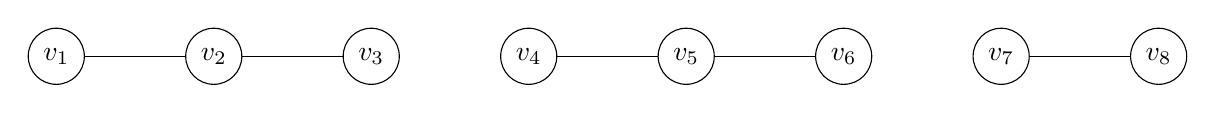
\begin{tikzpicture}[node distance={20mm}, main/.style = {draw, circle}] 
    \node[main] (1) {$v_1$};
    \node[main] (2) [right of=1] {$v_2$};
    \node[main] (3) [right of=2] {$v_3$};
    \node[main] (4) [right of=3] {$v_4$};
    \node[main] (5) [right of=4] {$v_5$};
    \node[main] (6) [right of=5] {$v_6$};
    \node[main] (7) [right of=6] {$v_7$};
    \node[main] (8) [right of=7] {$v_8$};

    \draw (1) -- (2);
    \draw (2) -- (3);
    \draw (4) -- (5);
    \draw (5) -- (6);
    \draw (7) -- (8);
\end{tikzpicture}
\end{center}
grazie al Teorema cinese del resto so che anche $d_2$ è lo score di un grafo.
Costruisco quindi un grafo $G$ con $score(G)=d_2$ utilizzando il Teorema dello
score:
\[\begin{array}{rccccccccccl}
    d_2  &= &(1, &1, &2, &2, &2, &3, &3, &3, &4, &5)\\
         &  &    &   &\downarrow& &  &\downarrow &\downarrow &\downarrow &\downarrow&\\
    d_2' &= &(1, &1, &1, &2, &2, &2, &2, &2, &3)\\
         &  &    &   &   &\downarrow &\downarrow &\downarrow\\
    d_2''&= &(1, &1, &1, &1, &1, &1, &2, &2)
\end{array}\]
\begin{center}
\hspace{-4cm}\begin{tikzpicture}[node distance={20mm}, main/.style={draw, circle}]
    \node[main] (1) {$v_1$};
    \node[main] (2) [right of=1] {$v_2$};
    \node[main] (3) [right of=2] {$v_3$};
    \node[main] (4) [right of=3] {$v_4$};
    \node[main] (5) [right of=4] {$v_5$};
    \node[main] (6) [right of=5] {$v_6$};
    \node[main] (7) [right of=6] {$v_7$};
    \node[main] (8) [right of=7] {$v_8$};
    \node[main] (9) [above of=4] {$v_9$};
    \node[main] (10) [above of=2] {$v_{10}$};

    \draw (1) -- (2);
    \draw (2) -- (3);
    \draw (4) -- (5);
    \draw (5) -- (6);
    \draw (7) -- (8);
    \draw (9) -- (3);
    \draw (9) -- (4);
    \draw (9) -- (6);
    \draw (10) -- (1);
    \draw (10) -- (2);
    \draw (10) -- (3);
    \draw (10) -- (9);

    \draw (10) to [out=180, in=215, looseness=3.2] (4);

    \node[font=\Large] (11) [above of=7] {G};
\end{tikzpicture}
\end{center}
La risposta alla questione (3a) è Sì, in quanto, il grafo $G$ che ho costruito ha
2 componenti connesse, quindi è sconnesso. Invece, la risposta alla questione
(3b) è No, in quanto i grafi 2-connessi non hanno foglie, mentre i grafi con
score $d_2$ ne hanno 2.

\newpage
\paragraph{Domanda di teoria}
Si enunci e si dimostri il Teorema di Fermat-Eulero e si dica come viene
utilizzato nella crittografia RSA.
\subparagraph{Enunciato Teorema di Fermat-Eulero:}
Sia $n\in\mathbb{N}$ con $n>0$. $\forall\alpha\in\inv$, vale:
\[\alpha^{\Phi(n)}=[1]_n\text{ in }\inv\]
o, equivalentemente, $\forall\alpha\in\mathbb{Z}\ t.c.\ (\alpha,n)=1$, vale:
\[\alpha^{\Phi(n)}\equiv1\Mod{n}\]
\begin{demonstration}
    Sia $\alpha\in\inv$. Si consideri la funzione:
    \[L_\alpha:\inv\to\inv\]
    tale che $L_\alpha(\beta)\mapsto\alpha\cdot\beta\ \forall\beta\in\inv$.
    Poiché dominio e codominio di $L_\alpha$ coincidono entrambi con $\inv$ che
    è un insieme finito, se riesco a dimostrare che $L_\alpha$ è una funzione
    iniettiva, allora varrà anche la suriettività. Dimostro l'iniettività di
    $L_\alpha$. Siano $\beta_1,\beta_2\in\inv$ tali che $L_\alpha(\beta_1)=L
    _\alpha(\beta_2)$. Provo che $\beta_1=\beta_2$. Vale:
    \[L_\alpha(\beta_1)=L_\alpha(\beta_2)\Leftrightarrow\alpha\cdot\beta_1=
    \alpha\cdot\beta_2\]
    poiché $\alpha\in\inv$, $\alpha$ è invertibile, ovvero esiste $\alpha^{-1}\in
    \inv$ tale che $\alpha\cdot\alpha^{-1}=[1]_n$. Dunque vale:
    \[\alpha\cdot\beta_1=\alpha\cdot\beta_2\Leftrightarrow\alpha^{-1}\cdot\alpha
    \cdot\beta_1=\beta_2\cdot\alpha\cdot\alpha^{-1}\Leftrightarrow[1]_n\cdot
    \beta_1=[1]_n\cdot\beta_2\Leftrightarrow\beta_1=\beta_2\]
    Quindi, $L_\alpha$ è una funzione iniettiva e suriettiva, dunque è una
    bigezione.

    Passo alla dimostrazione del teorema vero e proprio. Sia $n\in\mathbb{Z}$ con
    $n>0$ e sia $k\coloneqq\Phi(n)$. Se $\inv=\{\beta_1,\dots,\beta_k\}$, poiché
    $L_\alpha$ è una bigezione, i valori $L_\alpha(\beta_1),\dots,L_\alpha(\beta_k)$
    sono tutti e soli gli elementi di $\inv$ eventualmente riordinati. Per la
    commutatività del prodotto in $\inv$ vale:
    \[\prod_{i=1}^k\beta_i=\prod_{i=1}^kL_\alpha(\beta_1)=\prod_{i=1}^k\alpha
    \cdot\beta_i=\alpha^k\cdot\prod_{i=1}^k\beta_i\]
    Se $\inv\ni\gamma\coloneqq\prod_{i=1}^k\beta_i$, vale che:
    \[\gamma=\alpha^k\cdot\gamma\Leftrightarrow\gamma^{-1}\cdot\gamma=\alpha^k\cdot
    \gamma\cdot\gamma^{-1}\Leftrightarrow[1]_n=\alpha^k\cdot[1]_n\Leftrightarrow
    [1]_n=\alpha^k\]
    Ora, se $\alpha\in\mathbb{Z}$, vale anche che:
    \[[\alpha]^{\Phi(n)}_n=[1]_n\Rightarrow[\alpha^{\Phi(n)}]_n\Leftrightarrow
    \alpha^{\Phi(n)}\equiv1\Mod{n}\]
    La tesi del teorema è quindi verificata.
\end{demonstration}
Il Teorema di Fermat-Eulero viene usato per dimostrare il Teorema fondamentale
della crittografia RSA.
\subparagraph{Enunciato Teorema fondamentale della crittografia RSA:}
Siano $n,c\in\mathbb{N}\backslash0$. Se $(c,\Phi(n))=1$ e $d>0$ con $d\in[c]^{-1}
_{\Phi(n)}$, allora la funzione $P_c:\inv\to\inv$, tale per cui $P_c(\beta)
\mapsto\beta^c\ \forall\beta\in\inv$, è una funzione invertibile e vale:
\[\left(P_c\right)^{-1}=P_d\]
con $P_d:\inv\to\inv$ e tale che $P_d(\beta)=\beta^d\ \forall\beta\in\inv$.
\begin{demonstration}
    Sia $\alpha\in\inv$. Devo dimostrare che $P_d\left(P_c(\alpha)\right)=\alpha$.
    Poiché $d\in[c]^{-1}_{\Phi(n)}$, vale:
    \[c\cdot d\equiv1\Mod{n}\Leftrightarrow\Phi(n)|c\cdot d-1\Leftrightarrow
    \exists k\in\mathbb{Z}\ t.c.\ k\cdot\Phi(n)=c\cdot d-1\Leftrightarrow k\cdot
    \Phi(n)+1=c\cdot d\]
    Osservo che, $k\cdot\Phi(n)=c\cdot d-1$, ma per ipotesi $c,d>0$, dunque $c
    \cdot d-1\geq0$, inoltre $\Phi(n)>0$, quindi anche $k\geq0$. Per il Teorema
    di Fermat-Eulero $\alpha^k=[1]_n$, quindi vale:
    \[P_d\left(P_c(\alpha)\right)=P_d\left(\alpha^c\right)=\left(\alpha^c\right)
    ^d=\alpha^{c\cdot d}=\alpha^{1+k\cdot\Phi(n)}=\alpha\cdot\alpha^{k\cdot\Phi(n)}
    =\alpha\cdot\left(\alpha^{\Phi(n)}\right)^k=\alpha\cdot\left([1]_n\right)^k=
    \alpha\]
    Dunque la tesi del teorema è dimostrata.
\end{demonstration}
Il teorema appena dimostrato consente di utilizzare il metodo della crittografia
RSA per crittografare e decriptare messaggi. Il metodo RSA funziona come segue:

Siano $\alpha$ il messaggio da trasmettere, $M$ e $D$ mittente e destinatario.
Il valore c, detto chiave pubblica e noto a tutti, è utilizzato soltanto per
crittografare i messaggi da $M$ a $D$. Soltanto $D$ conosce il valore $d$, detto
chiave privata, necessario per decriptare tali messaggi. Al momento dell'invio
$M$ calcola $P_c(\alpha)$ e ne trasmette il risultato. $D$ riceve $P_c(\alpha)$
e calcola $P_d\left(P_c(\alpha)\right)$.

Grazie al Teorema fondamentale della crittografia RSA,
$P_d\left(P_c(\alpha)\right)=\alpha$, per cui $D$ può leggere il messaggio.

\end{document}